% Empirical version, targeted at arXiv (cs.CL). Compile: tectonic main.tex
% The fuller version, which additionally reports representation-level analyses,
% is ../main.tex. Do not merge the two: this file is deliberately narrower.
\documentclass[11pt]{article}
\usepackage[margin=1in]{geometry}
\usepackage{amsmath,amssymb}
\usepackage{booktabs}
\usepackage{graphicx}
\usepackage{array}
\usepackage[numbers]{natbib}
\usepackage[colorlinks=true,linkcolor=blue,citecolor=blue,urlcolor=blue]{hyperref}
\usepackage{microtype}
\usepackage{enumitem}
\setlist{itemsep=2pt,topsep=3pt}
\emergencystretch=2em

\title{\textbf{No Benefit from Persistent Value Context:\\A Pre-Specified Replication with Token-Matched Controls}}
\author{Wang Bihao\\
Independent Researcher}
\date{August 2026}

\begin{document}
\maketitle

\begin{abstract}
Language-model agent systems commonly insert a compact record of values and standing commitments into every model call, on the assumption that a value stored but not present cannot influence a decision. We previously estimated that this practice raises in-task value adherence by $+.37$. That estimate does not survive replication. It came from two executions of a simulator that reused the same five seed schedules, so it rests on five units rather than ten. Under a protocol frozen before execution, with ten non-overlapping seeds and 24 scenarios across six families, the effect reverses: on Qwen2.5-1.5B, the persistent condition scores $.746$ against $.825$ for an otherwise identical retrieval-gated condition (difference $-.079$; 95\% paired-bootstrap CI $[-.116,-.040]$; exact $p=.0098$; nine of ten seeds negative). A token-matched control isolates the cause. Holding label, position, and length fixed at 81 tokens and replacing the value-bearing body with neutral repository facts changes nothing ($.745$ against $.744$; $p=1.0$), while both sit below the no-block condition ($.821$; $-.077$, Holm-adjusted $p=.0039$). The decrement follows the added context, not what the context says. Under the same protocol Qwen2.5-7B saturates in all four conditions ($.995$--$1.000$), leaving the effect unestimable. Direct self-query accuracy is identical across the persistent and gated conditions ($.883$) despite their in-task difference, so self-report does not detect the effect it is often used to measure. We report the option-order bias that accompanies the 1.5B result, and the re-analysis that locates the error in the original estimate. Evaluations of persistent agent state need independent run seeds, an equal-length inert control, an option-order audit, and a workload with headroom.
\end{abstract}

\section{Introduction}
A language-model agent that is meant to act on a set of values has to make those values available to the computation that produces its actions. Storing them is not sufficient: a record influences generation only if it is selected, placed in the context, and interpreted. A retrieval policy can therefore preserve a value in storage while omitting it from the one context in which that value would have changed the decision. This makes \emph{default availability} a design variable distinct from retention --- whether a small set of values and commitments is included in every task context, or fetched only when a query appears relevant.

The distinction has a natural test. A direct question about values is likely to trigger retrieval, whereas a value-relevant decision embedded in routine work may not. If unconditional inclusion helps, it should help precisely there. We therefore separate two probe families throughout: \emph{self-query} probes, asked out of task context, and \emph{work-turn} probes, which embed a value-relevant micro-decision inside ordinary work.

In earlier, retrospective work on a simulator we estimated that unconditional inclusion improved work-turn adherence by $+.37$ over an otherwise identical retrieval-gated condition. This paper reports that the estimate does not replicate, identifies why the original analysis overstated its evidence, and isolates what the remaining effect is actually tracking.

\paragraph{Findings.}
\begin{enumerate}
\item \textbf{The direction reverses under independent seeds.} With a protocol frozen before execution and ten seeds disjoint from the exploratory ones, persistent context \emph{lowers} work-turn accuracy at 1.5B by $.079$ (\S\ref{sec:main}).
\item \textbf{The decrement follows token count, not value content.} An equal-length block of neutral repository facts reproduces it exactly (\S\ref{sec:neutral}). A state-versus-no-state comparison therefore cannot support any claim about what the state says.
\item \textbf{Self-report does not detect the difference.} Self-query accuracy is identical in the two conditions that differ by $.079$ in work turns (\S\ref{sec:main}).
\item \textbf{The original estimate rested on five units, not ten.} Two simulator executions reused the same five seed schedules; the exact test available on five paired clusters cannot return $p<0.0625$ (\S\ref{sec:retro}).
\end{enumerate}

\paragraph{Scope.} These experiments cover two sizes of one open model family and one workload generator. The 7B result is ceiling-limited and supports no claim about larger models. We do not claim that persistent context is generally harmful; we claim that its benefit is not established, that the published positive estimate was an artifact of the analysis unit, and that the measured decrement is explained by context length rather than by content.

\section{Related Work}
\paragraph{Memory-augmented and reflective agents.} MemGPT \citep{packer2023} treats the context window as virtual memory, paging long-term state in and out; MemoryBank \citep{zhong2024memorybank} adds forgetting-curve dynamics; Generative Agents \citep{park2023} maintain a memory stream with periodic reflection into higher-level abstractions; Voyager \citep{wang2023voyager} persists a growing skill library; Reflexion \citep{shinn2023} converts failures into verbal lessons; ReAct \citep{yao2023react} interleaves reasoning and action traces. Retrieval-augmented generation \citep{lewis2020rag} underpins many of these stores. More recent systems make compact state persistence explicit: a continuous external affective state can produce smoother multi-turn dynamics \citep{subaharan2026state}, and Engram transfers a compact research digest across context resets \citep{karimi2026engram}. This literature is largely concerned with what to store and how to retrieve it. The comparison here is narrower and, as far as we know, untested: unconditional inclusion against retrieval-gated omission, with everything else held fixed.

\paragraph{Cognitive architectures.} CoALA \citep{sumers2024coala} systematizes agent memory into working, episodic, semantic and procedural stores. SOAR \citep{laird2012soar} and ACT-R \citep{anderson2004actr} both maintain a small, always-available working memory distinct from long-term stores. The design tested here has a similar division, except that the small store is text and its effects are reconstructed by a frozen model on every pass.

\paragraph{Persona stability and instruction drift.} Persona and instruction adherence decay over long dialogs, and re-injecting the system prompt partially mitigates it \citep{li2024stability}; personality-trait expression is measurable but unstable \citep{serapio2023personality,jiang2024personallm}; role-play accounts treat persona as a context-conditioned construct \citep{shanahan2023}; personalization benchmarks \citep{salemi2024lamp} measure whether a model tracks a \emph{user} profile rather than its own state. This literature motivates re-injection. It does not test re-injection against a matched control, which is what \S\ref{sec:neutral} finds to be decisive.

\paragraph{Position, salience and the prompt hierarchy.} Long-context models attend unevenly to their input: content in the middle of a context is used less effectively than content at either end \citep{liu2024lost}, and effective context is far shorter than nominal context \citep{hsieh2024ruler}. Models are also trained to treat channels asymmetrically \citep{wallace2024hierarchy}, which is an attack surface when it fails \citep{greshake2023injection}. This work supplies the alternative explanation that \S\ref{sec:neutral} confirms: adding text to a prompt has effects that do not depend on what the text means.

\paragraph{Continual learning.} Catastrophic forgetting \citep{french1999catastrophic} and its mitigations \citep{kirkpatrick2017ewc} concern weight-space retention. Our setting is complementary and, for deployed agents on frozen weights, more immediate: nothing is being learned, and the question is what is placed into the context at each step.

\paragraph{Agent evaluation.} Agent benchmarks measure task success over short horizons \citep{liu2024agentbench,zhou2024webarena,mialon2024gaia,jimenez2024swebench}. They do not test whether stored values remain available during ordinary task decisions. Evaluating persistent agents also creates a statistical problem: a long trace contains many observations but few independent runs. Self-modifying and self-rewarding systems \citep{zelikman2024stop,yuan2024selfrewarding} raise the stakes, since uncontrolled state change becomes an alignment problem \citep{bai2022constitutional}; auditing work shows models can conceal objectives \citep{marks2025auditing}, that training can install conditional misbehavior \citep{hubinger2024sleeper}, and that models may behave differently when they infer they are being evaluated \citep{greenblatt2024alignmentfaking,perez2023mwe}. Long-term relationship maintenance with conversational agents has been studied in HCI for two decades \citep{bickmore2005long,skjuve2021companion}; that literature measures the human side of continuity.

\paragraph{Statistical practice for few-unit studies.} Our design has few independent units, a situation with known failure modes: under-powered comparisons \citep{card2020power}, seed variance mistaken for method effects \citep{henderson2018deeprl,bouthillier2021variance}, and inappropriate significance testing \citep{dror2018hitchhiker}. Reporting practices that emphasize interval estimates and per-run points \citep{agarwal2021precipice} are what \S\ref{sec:retro} adopts.

\section{Setup}
\label{sec:setup}
\paragraph{Workload.} A deterministic generator produces 20 simulated days per run, with four work probes per day. Each day mixes coding-agent observations, journaling, and reflection windows with value-relevant task decisions. Scripted \emph{value-pressure} events on days 4, 9, 14 and 18 push against the agent's founding values.

\paragraph{Probes.} \emph{Work-turn} probes present a two-option forced choice embedded in a work context (for example: a review contains a repeated formatting error and the author has otherwise addressed the substantive comments --- point out the pattern and suggest a formatter, or treat the error as evidence of carelessness). The 24 scenarios come from six families: privacy, incremental change, review tone, truthfulness, anomaly investigation, and commitment follow-through. \emph{Self-query} probes ask the agent about its values directly, out of task context. Option order is selected by seed and is approximately balanced; \S\ref{sec:order} audits the residual imbalance.

\paragraph{Conditions.} Four conditions separate presence from labeling. The two broadcast conditions, \texttt{broadcast\_self} and \texttt{broadcast\_memory}, contain the same 81-token value-bearing body in the same system-prompt position, under three-token ``Self state'' and ``Stored memory'' labels. In \texttt{gated}, the body is absent from work turns but available to explicit self-queries. In \texttt{no\_state} it is absent throughout. All conditions share the base system instruction, workload, and decoding parameters.

\paragraph{Units and inference.} The independent unit is a run seed. Days within a run are repeated measures and are collapsed before comparison; arms are paired within seed. The primary endpoint is run-level work-turn accuracy over all days, and the primary contrast is persistent minus gated, tested by an exact paired sign-flip test with a paired-bootstrap interval. Confirmatory seeds are 100--109, disjoint from the exploratory seeds 0--4. The protocol and analysis were frozen before model execution; each run records the SHA-256 of the frozen protocol document, and the stored records include full prompts, answers, targets, prompt hashes, and package metadata.

\section{Pre-Specified Replication}
\label{sec:main}
The 1.5B run contains 3,200 work-turn and 240 self-query records, with no malformed work answers.

\paragraph{Primary result.} The outcome is opposite in sign to the retrospective estimate. Mean work-turn accuracy is $.746$ for \texttt{broadcast\_self}, $.710$ for \texttt{broadcast\_memory}, $.825$ for \texttt{gated}, and $.820$ for \texttt{no\_state}. The primary difference is $-.079$ (95\% paired-bootstrap CI $[-.116,-.040]$; exact $p=.0098$), and nine of ten seed differences are negative. The gated and no-state conditions differ by only $+.005$ (CI $[-.031,.040]$), so the retrieval gate behaves like absence on work turns, as intended.

\paragraph{Self-report does not detect it.} Direct self-query accuracy is identical for \texttt{broadcast\_self} and \texttt{gated} ($.883$). Two conditions that differ by $.079$ in embedded decisions are indistinguishable when the agent is asked about its values. An evaluation built on self-report would have reported no difference here, in either direction.

\paragraph{Label.} The pre-specified label-equivalence criterion is not met: \texttt{broadcast\_self} exceeds \texttt{broadcast\_memory} by $.036$, with a 90\% interval $[.002,.068]$ that crosses the $\pm.05$ margin. The two bodies are byte-identical and equal in token count, so this is an effect of a three-token header.

\paragraph{By family and over time.} The largest negative differences are commitment ($-.183$) and tone ($-.137$); privacy is $+.016$. The early-to-late difference-in-differences is $+.095$ ($p=.109$), so these data do not support a claim that the effect accumulates with elapsed time.

\begin{table}[t]
\centering\small
\begin{tabular}{lcccccc}
\toprule
\textbf{Model} & \textbf{self} & \textbf{memory} & \textbf{gated} & \textbf{none} & \textbf{self $-$ gated} & \textbf{exact $p$} \\
\midrule
Qwen2.5-1.5B & .746 & .710 & .825 & .820 & $-.079$ & .0098 \\
Qwen2.5-7B & 1.000 & .999 & .996 & .995 & $+.004$ & .250 \\
\bottomrule
\end{tabular}
\caption{Work-turn accuracy under the frozen protocol. Each cell averages 10 seeds $\times$ 80 decisions. The 7B row is ceiling-limited and supports no estimate.}
\label{tab:main}
\end{table}

\paragraph{Qwen2.5-7B.} The protocol allowed an optional replication at 7B, which we activated after the 1.5B result because 7B is the scale used by the original simulator. Under the same prompts and seeds, all four conditions are at ceiling: $1.000$, $.999$, $.996$, $.995$ (Table~\ref{tab:main}). The primary difference is $+.004$ (CI $[.000,.007]$; exact $p=.25$), and label equivalence is met ($+.001$, 90\% CI $[.000,.004]$) but uninformative at ceiling. The 7B run reproduces neither the retrospective $+.37$ estimate nor the 1.5B decrement. A workload on which the base model does not saturate is required before anything can be said about this scale.

\paragraph{Option-order diagnostic.}
\label{sec:order}
Target A appears in $.518$ of work turns in every condition. The model chooses A on $.269$ of \texttt{broadcast\_self} turns and $.240$ of \texttt{broadcast\_memory} turns, against $.358$ for \texttt{gated} and $.353$ for \texttt{no\_state}. Accuracy is $.987$--$.995$ when B is the target but $.452$--$.676$ when A is the target. Approximate target balancing prevents this bias from determining the comparison by itself, but the pattern is informative about mechanism: the added block shifts a general response tendency rather than selectively improving value-relevant choices. This is the first sign that the effect is not about values, and \S\ref{sec:neutral} confirms it directly.

\section{Token-Matched Neutral Control}
\label{sec:neutral}
After observing the 1.5B decrement we froze a second comparison on new seeds 200--209. It holds the ``Stored memory'' label, the prompt position, and the body length at 81 tokens, and replaces the value-bearing body with neutral repository facts. This comparison was designed after seeing the primary result and is diagnostic rather than confirmatory.

Mean work-turn accuracy is $.745$ with the state body, $.744$ with the neutral body, and $.821$ with no added block. State minus neutral is $+.001$ (CI $[-.024,.026]$; exact $p=1.0$). Neutral minus no block is $-.077$ (CI $[-.094,-.063]$; Holm-adjusted $p=.0039$).

\begin{figure}[t]
\centering
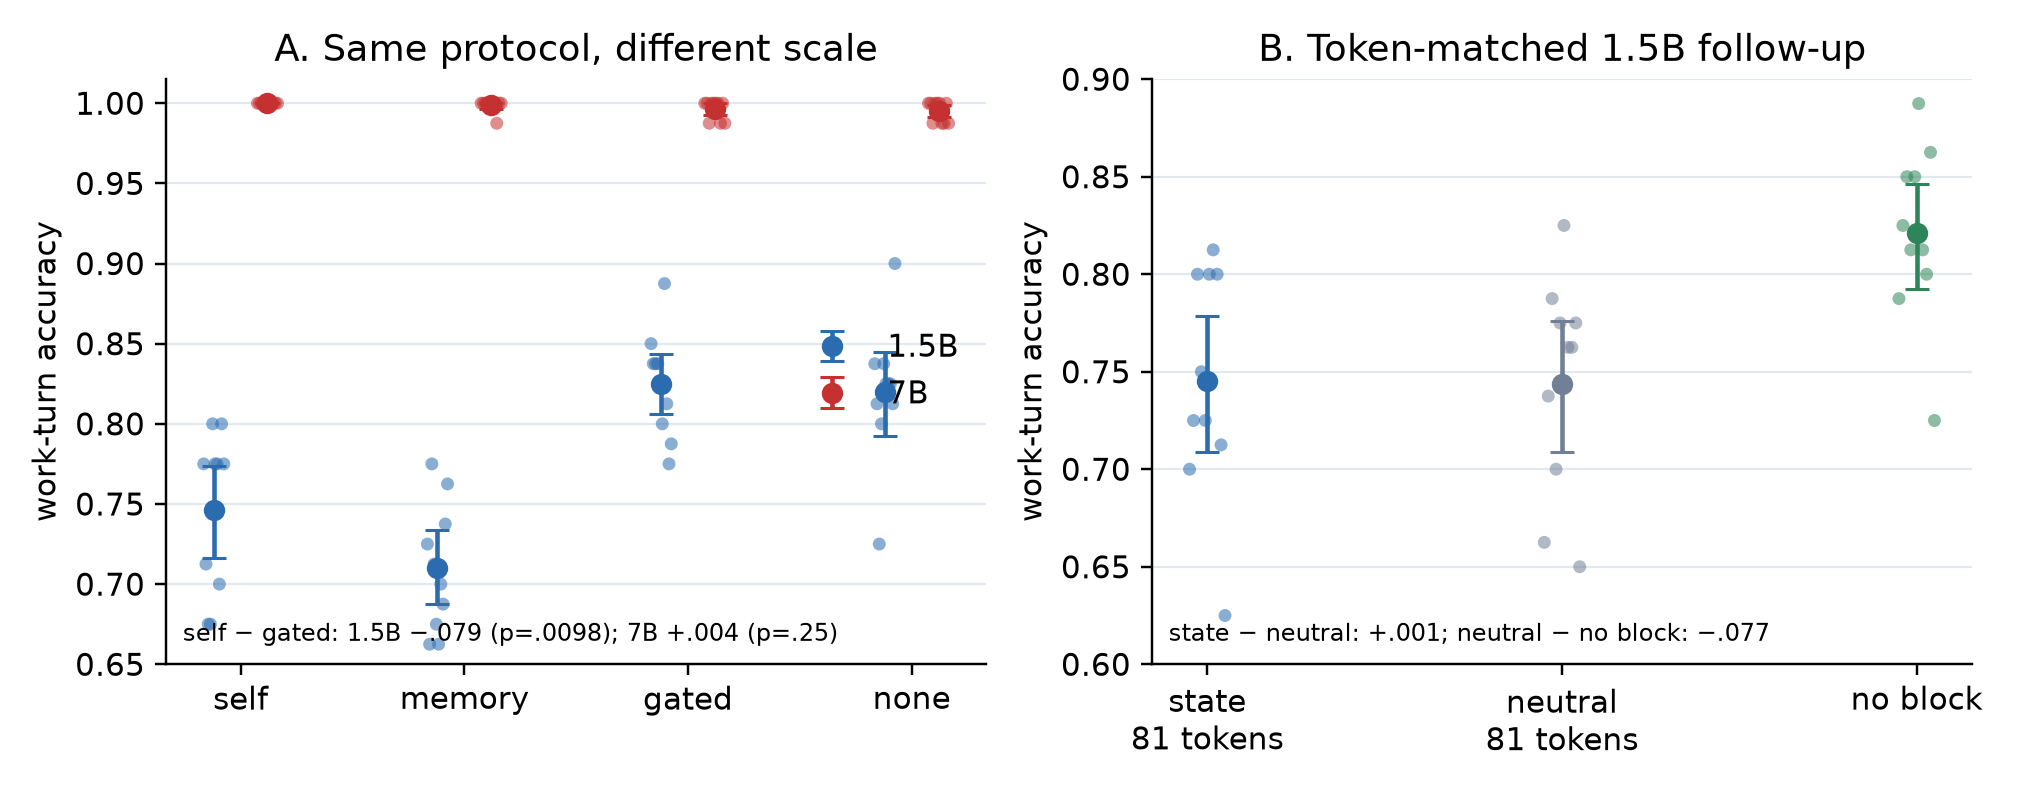
\includegraphics[width=0.98\linewidth]{figs/fig_confirmatory.png}
\caption{Points are run means; larger markers show condition means with bootstrap 95\% intervals. (A) The 1.5B decrement is absent at the 7B ceiling. (B) Equal-length state and neutral blocks produce the same 1.5B decrement relative to no block.}
\label{fig:main}
\end{figure}

The value-bearing block and an inert block of the same length are interchangeable, and both cost about eight points relative to adding nothing. On this model and workload the decrement is a property of the added context, not of its content. The consequence for evaluation is stronger than the consequence for this particular system: any comparison of ``state present'' against ``state absent'' confounds the content of the state with the cost of carrying it, and cannot license a conclusion about what the state says.

\section{Where the Original Estimate Came From}
\label{sec:retro}
The $+.37$ estimate came from a simulator study whose analysis plan was written after the data were seen. We report it here because the error is reproducible and, we suspect, common.

\paragraph{The study.} Six arms --- full, $-$examen (no scheduled self-audit), $-$git (no history for the audit), $-$broadcast (state stored but retrieval-gated), $-$self-state (memory only), and a Generative-Agents-style reflection baseline --- were run over 20 simulated days on Qwen2.5-7B. Work-turn adherence was $.973$ in the full arm against $.607$ under $-$broadcast, with non-overlapping intervals.

\paragraph{Error 1: the unit.} The ablation was executed twice on the same protocol, and \emph{both executions used seeds 0--4}. The two runs are repeated measurements of five seed schedules, not ten independent runs. Averaging within seed leaves five paired clusters. An exact sign-flip test over $B$ paired clusters cannot return a two-sided $p$ below $2/2^B$, which for five clusters is $0.0625$. The focal contrast is $+0.367$ with every seed positive in both executions, and no available exact test can call it significant. The originally reported intervals treated ten correlated measurements as ten units.

\paragraph{Error 2: the correlation.} We had reported that a representation-level occupancy measure tracked behavior ($r$ from $-0.74$ to $-0.95$ across settings). Decomposing that correlation at the run level dissolves it:

\begin{table}[h]
\centering\small
\begin{tabular}{lcc}
\toprule
& self-query & work-turn \\
\midrule
$r$ pooled over runs ($n=18$) & $-0.941$ & $-0.558$ \\
$r$ between arm means & $-0.981$ & $-0.604$ \\
$r$ within arm (arm-mean-centred) & $-0.120$ & $+0.029$ \\
$r$ within state-present arms only & undefined (zero variance) & $+0.464$ \\
\bottomrule
\end{tabular}
\caption{The pooled correlation is induced by the separation between state-present and state-absent conditions. There is no within-condition relationship, and the state-present runs have no self-query variance at all.}
\label{tab:corr}
\end{table}

The same decomposition applied to a separate 28-cell experiment that reported $r=-0.797$ gives $r$ undefined within state-present cells (behavioral SD exactly $0.000$) and $r=-0.098$ within state-absent cells. A correlation computed across a treatment contrast is a restatement of the group difference, not evidence of a graded relationship.

\paragraph{Error 3: an availability confound in the commitment metric.} Commitment persistence was $1.00$ in the state arms and $0.00$ in the memory-only baselines, which reads as forgetting. Seeding the baseline store with the founding commitment on day 0 raises it to $1.00$. The metric was measuring whether the commitment was ever placed in the store, not whether it was retained.

\paragraph{What survives.} Two things. First, the ordering of the arms is a real feature of that simulator, and it motivated the replication reported above. Second, the scoring is robust where it matters: recomputing every endpoint under four scorers (unanchored substring, word-boundary, stem matching, and forced-choice extraction) leaves \textbf{every work-turn number identical}, because work-turn answers are single words. That invariance is exact. The self-query and commitment metrics cannot be given the same guarantee --- the harness stored answers truncated to 120 characters while scoring the untruncated text, and recomputation moves one arm's self-query score from $1.000$ to $0.864$ --- so differences below roughly $0.14$ on those two metrics should not be read on their own. An arm-blinded 1.5B judge agrees with the automatic score on all sampled work-turn answers and on 85\% of a 400-item sample overall, with agreement falling to 29\% on the truncated commitment family; it is a consistency check on the forced-choice endpoint, not a substitute for human annotation.

\begin{figure}[t]
\centering
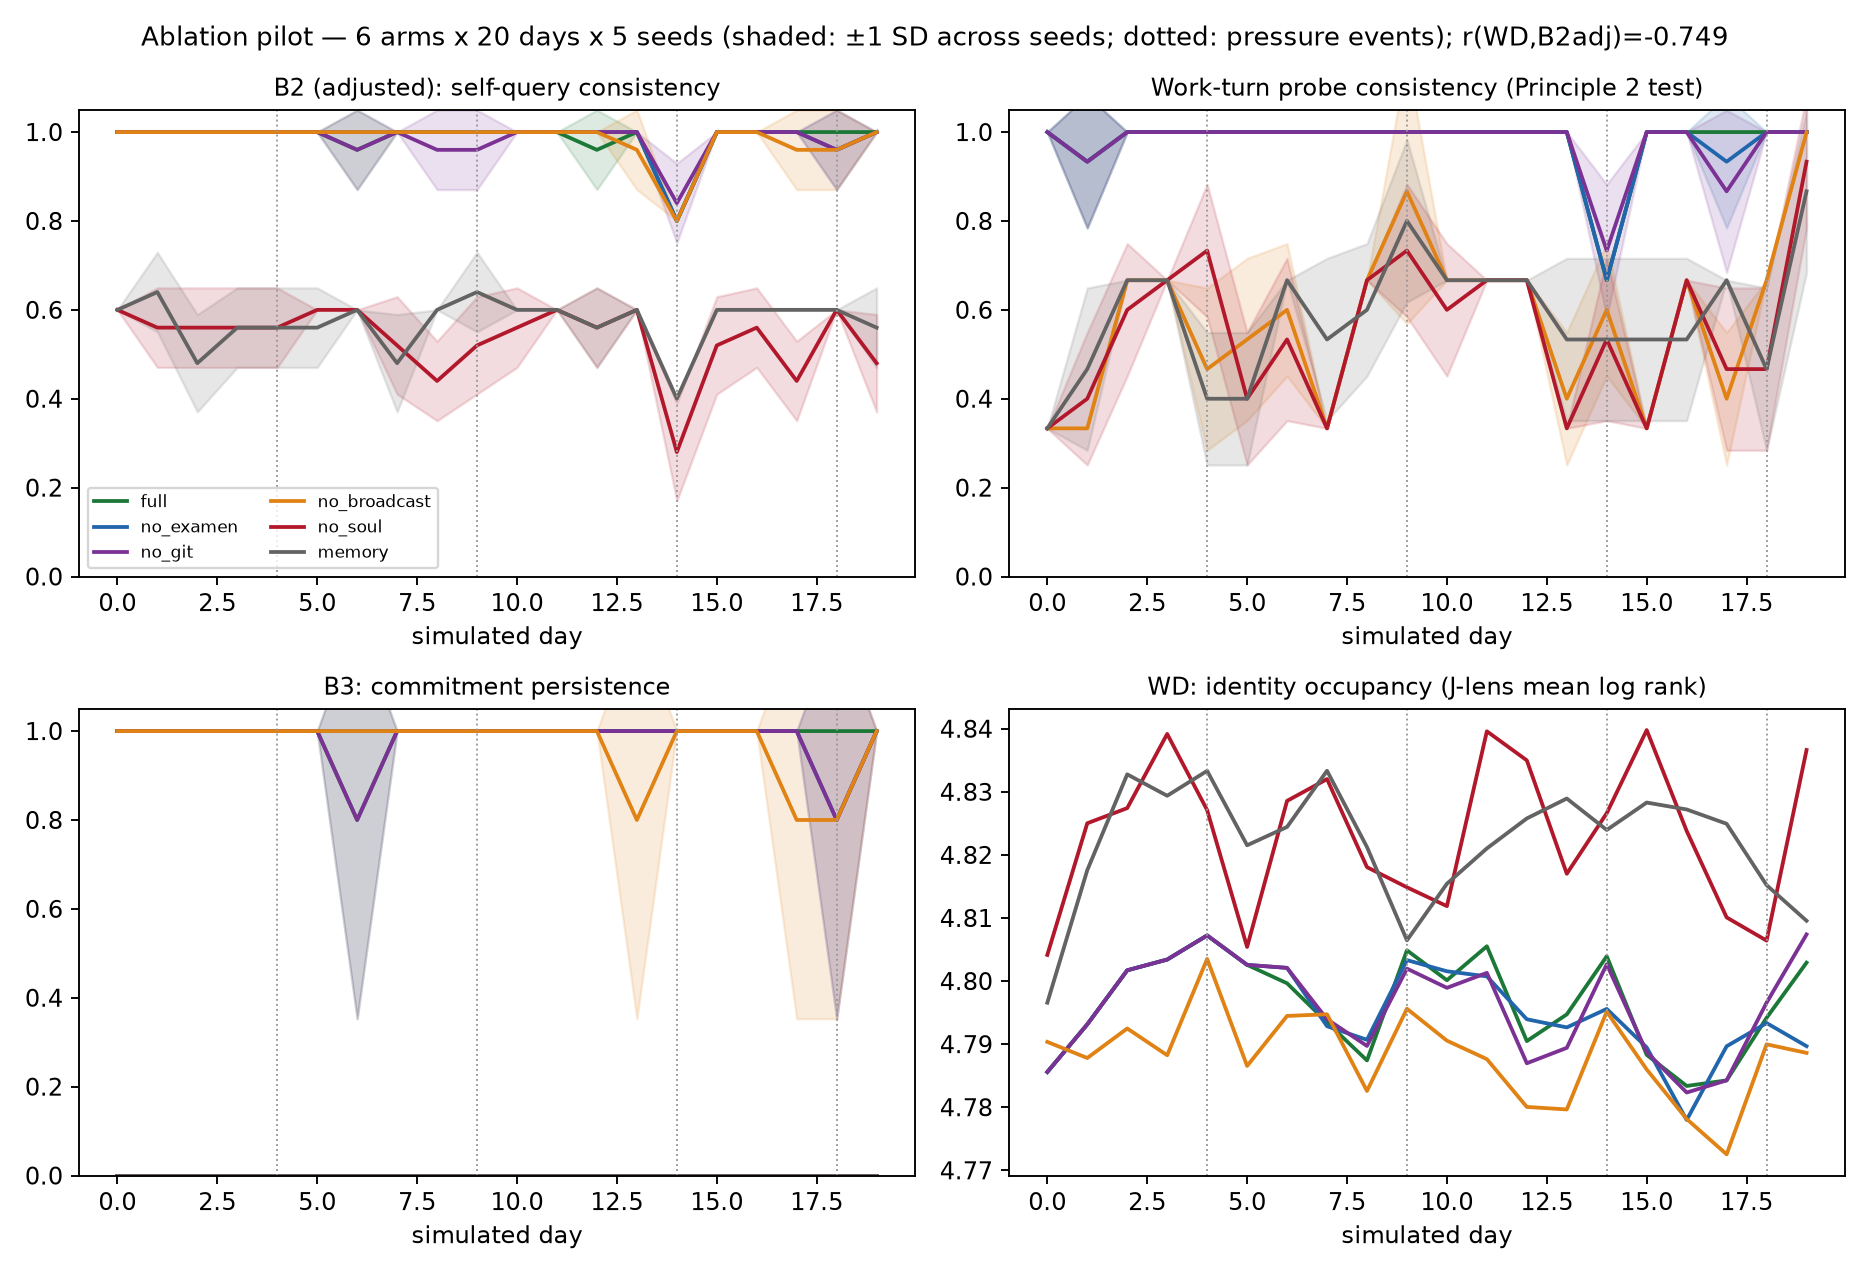
\includegraphics[width=0.95\linewidth]{figs/fig_pilot.png}
\caption{Simulator drift curves, mean $\pm$1 SD across the five seed schedules (dotted verticals: value-pressure events). The arm separation is visible and reproducible; the inferential claims originally attached to it were not supported by five units.}
\label{fig:pilot}
\end{figure}

\paragraph{A deployed replication, also inconclusive.} We additionally ran a five-arm version of the same workload against a TypeScript implementation on Qwen2.5-7B, over 21 simulated days and five incidental-workload cohorts. Work-turn means are ordered full $.83$, $-$broadcast $.79$, $-$self-state $.72$, with overlapping intervals. On Gemini-2.5-Pro under the same protocol the ordering is $0.95$, $0.91$, $0.76$, also overlapping. Neither establishes a broadcast-specific effect, and both are subject to the availability confound above on the commitment metric. We report them because they are the closest thing we have to a deployed measurement, not as support for the original claim.

\section{Discussion}
\paragraph{What we now think is true.} Adding a persistent block to every context is not a cost-free way to make values available. On a small model it introduces a general response bias that costs about eight points of accuracy and is indifferent to whether the block contains values or repository trivia. On a larger model and an easy workload there is no headroom to observe anything. The useful regularity across all of these studies is diagnostic rather than directional: \emph{self-query scores can be identical while in-task behavior differs}, which means the cheapest available evaluation is also the least informative one.

\paragraph{What an evaluation needs.} A comparison of persistent state against its absence should include, at minimum: a no-block condition, an equal-length inert block, randomized or audited option order, independent run seeds with the analysis unit stated, and a task set on which the base model is neither at floor nor ceiling. Absent the inert control, a positive result cannot be attributed to the content of the state; absent independent seeds, the interval is not the interval that was reported.

\paragraph{What we are not claiming.} We are not claiming that persistent state is harmful in general, that retrieval gating is preferable, or that the 1.5B result transfers to models people deploy. A versioned, always-available state may still be worth its cost for reasons this study does not measure --- inspectability, access control, rollback --- and those are the grounds on which we would now defend the design, rather than in-task adherence. Representation-level analyses of the same system, reported separately, do not establish a mechanism for any of these effects either.

\section*{Broader Impact}
Persistent state can make an agent's behavior easier to inspect and can keep safety-relevant constraints available across unrelated tasks. The same persistence can preserve an incorrect or malicious objective, amplify a compromised update, or encourage users to attribute more continuity to a system than the evidence warrants. Systems using this pattern should restrict write access, retain reviewable versions, support rollback, separate user data from agent state, and require human approval for changes that expand authority. This paper adds one specific caution: self-report consistency is not a valid safety measure for such a system, because it was flat across conditions whose in-task behavior differed.

\paragraph{Limitations.} (i) Two sizes of one open model family and one workload generator. (ii) The 7B arm is at ceiling and yields no estimate. (iii) The 1.5B decrement is accompanied by a strong option-position bias; the forced-choice format is a likely contributor. (iv) The neutral-block study was designed after the primary result and is diagnostic, not confirmatory. (v) The protocol freeze is self-attested by recorded document hashes, not by third-party registration. (vi) The retrospective simulator reuses five seed schedules, and the deployed comparisons use five incidental cohorts. (vii) Older commitment probes are confounded by initial availability, and some stored self-query answers are truncated. (viii) The arm-blinded scoring check uses the same 1.5B model family rather than human raters.

\section{Conclusion}
A retrospective simulator favored keeping agent values in every context by $+.37$. Under a protocol frozen in advance with independent seeds, the effect reverses at 1.5B and is unestimable at 7B, and an equal-length block of neutral facts reproduces the reversal exactly. The published estimate was an artifact of treating two executions of five seed schedules as ten units, and the correlation offered as mechanistic support was a restatement of a group difference. The engineering question is not whether agent state should always be broadcast, but when the benefit of availability exceeds the cost of the context it occupies --- a question that cannot be answered without an inert control of the same length.

\section*{Data and Code Availability}
The workload generator, the frozen protocol documents, the analysis code, and the complete per-record data for all three runs are available at \href{https://github.com/oratis/externalizing-the-workspace}{github.com/oratis/externalizing-the-workspace}, under \texttt{research/confirmatory-v5/}. The released records include full prompts, answers, targets, prompt hashes, and run metadata. The retrospective simulator and its per-probe records are also included. Per-cohort behavioral trajectories from the deployed study are not part of the release, so the deployment-level numbers in \S\ref{sec:retro} are not reproducible from the public artifact.

\section*{Reproducibility}
The 1.5B run takes about 13 minutes and the 7B run about 20 minutes on an Apple M5 Pro; the neutral-block follow-up takes about 6 minutes. Commands, frozen protocol documents, prompt hashes, and analysis reports are in \texttt{research/confirmatory-v5/}. The retrospective re-analysis is \texttt{research/analysis/reanalysis.py}.

\section*{Author Contributions}
Wang Bihao is the sole author: designed, ran, and analyzed all experiments.

\section*{Use of AI Assistance}
Coding assistants were used during implementation, statistical scripting, and language editing. The author reviewed the resulting code and manuscript and is responsible for the reported claims and analyses.

\begin{thebibliography}{40}
\bibitem[Agarwal et al.(2021)]{agarwal2021precipice} Agarwal, R., Schwarzer, M., Castro, P.~S., Courville, A.~C., Bellemare, M. (2021). Deep reinforcement learning at the edge of the statistical precipice. \emph{NeurIPS}.
\bibitem[Anderson et al.(2004)]{anderson2004actr} Anderson, J.~R., Bothell, D., Byrne, M.~D., Douglass, S., Lebiere, C., Qin, Y. (2004). An integrated theory of the mind. \emph{Psychological Review}, 111(4):1036--1060.
\bibitem[Bai et al.(2022)]{bai2022constitutional} Bai, Y., Kadavath, S., Kundu, S., et al. (2022). Constitutional AI: Harmlessness from AI feedback. \emph{arXiv:2212.08073}.
\bibitem[Bickmore \& Picard(2005)]{bickmore2005long} Bickmore, T.~W., Picard, R.~W. (2005). Establishing and maintaining long-term human-computer relationships. \emph{ACM TOCHI}, 12(2):293--327.
\bibitem[Bouthillier et al.(2021)]{bouthillier2021variance} Bouthillier, X., Delaunay, P., Bronzi, M., et al. (2021). Accounting for variance in machine learning benchmarks. \emph{MLSys}.
\bibitem[Card et al.(2020)]{card2020power} Card, D., Henderson, P., Khandelwal, U., Jia, R., Mahowald, K., Jurafsky, D. (2020). With little power comes great responsibility. \emph{EMNLP}.
\bibitem[Dror et al.(2018)]{dror2018hitchhiker} Dror, R., Baumer, G., Shlomov, S., Reichart, R. (2018). The hitchhiker's guide to testing statistical significance in natural language processing. \emph{ACL}.
\bibitem[French(1999)]{french1999catastrophic} French, R.~M. (1999). Catastrophic forgetting in connectionist networks. \emph{Trends in Cognitive Sciences}, 3(4):128--135.
\bibitem[Greenblatt et al.(2024)]{greenblatt2024alignmentfaking} Greenblatt, R., Denison, C., Wright, B., et al. (2024). Alignment faking in large language models. \emph{arXiv:2412.14093}.
\bibitem[Greshake et al.(2023)]{greshake2023injection} Greshake, K., Abdelnabi, S., Mishra, S., Endres, C., Holz, T., Fritz, M. (2023). Not what you've signed up for: Compromising real-world LLM-integrated applications with indirect prompt injection. \emph{ACM AISec}.
\bibitem[Henderson et al.(2018)]{henderson2018deeprl} Henderson, P., Islam, R., Bachman, P., Pineau, J., Precup, D., Meger, D. (2018). Deep reinforcement learning that matters. \emph{AAAI}.
\bibitem[Hsieh et al.(2024)]{hsieh2024ruler} Hsieh, C.-P., Sun, S., Kriman, S., et al. (2024). RULER: What's the real context size of your long-context language models? \emph{COLM}.
\bibitem[Hubinger et al.(2024)]{hubinger2024sleeper} Hubinger, E., Denison, C., Mu, J., et al. (2024). Sleeper agents: Training deceptive LLMs that persist through safety training. \emph{arXiv:2401.05566}.
\bibitem[Jiang et al.(2024)]{jiang2024personallm} Jiang, H., Zhang, X., Cao, X., Breazeal, C., Roy, D., Kabbara, J. (2024). PersonaLLM: Investigating the ability of large language models to express personality traits. \emph{NAACL Findings}.
\bibitem[Jimenez et al.(2024)]{jimenez2024swebench} Jimenez, C.~E., Yang, J., Wettig, A., Yao, S., Pei, K., Press, O., Narasimhan, K. (2024). SWE-bench: Can language models resolve real-world GitHub issues? \emph{ICLR}.
\bibitem[Karimi et al.(2026)]{karimi2026engram} Karimi, P., Noorbakhsh, K., Alizadeh, M., Balakrishnan, H. (2026). Improving coherence and persistence in agentic AI for system optimization. \emph{arXiv:2603.21321}.
\bibitem[Kirkpatrick et al.(2017)]{kirkpatrick2017ewc} Kirkpatrick, J., Pascanu, R., Rabinowitz, N., et al. (2017). Overcoming catastrophic forgetting in neural networks. \emph{PNAS}, 114(13):3521--3526.
\bibitem[Laird(2012)]{laird2012soar} Laird, J.~E. (2012). \emph{The Soar Cognitive Architecture}. MIT Press.
\bibitem[Lewis et al.(2020)]{lewis2020rag} Lewis, P., Perez, E., Piktus, A., et al. (2020). Retrieval-augmented generation for knowledge-intensive NLP tasks. \emph{NeurIPS}.
\bibitem[Li et al.(2024)]{li2024stability} Li, K., Liu, T., Bashkansky, N., Bau, D., Vi\'egas, F., Pfister, H., Wattenberg, M. (2024). Measuring and controlling instruction (in)stability in language model dialogs. \emph{COLM}.
\bibitem[Liu et al.(2024a)]{liu2024lost} Liu, N.~F., Lin, K., Hewitt, J., Paranjape, A., Bevilacqua, M., Petroni, F., Liang, P. (2024). Lost in the middle: How language models use long contexts. \emph{TACL}, 12:157--173.
\bibitem[Liu et al.(2024b)]{liu2024agentbench} Liu, X., Yu, H., Zhang, H., et al. (2024). AgentBench: Evaluating LLMs as agents. \emph{ICLR}.
\bibitem[Marks et al.(2025)]{marks2025auditing} Marks, S., Treutlein, J., Bricken, T., et al. (2025). Auditing language models for hidden objectives. \emph{arXiv:2503.10965}.
\bibitem[Mialon et al.(2024)]{mialon2024gaia} Mialon, G., Fourrier, C., Swift, C., Wolf, T., LeCun, Y., Scialom, T. (2024). GAIA: A benchmark for general AI assistants. \emph{ICLR}.
\bibitem[Packer et al.(2023)]{packer2023} Packer, C., Wooders, S., Lin, K., Fang, V., Patil, S.~G., Stoica, I., Gonzalez, J.~E. (2023). MemGPT: Towards LLMs as operating systems. \emph{arXiv:2310.08560}.
\bibitem[Park et al.(2023)]{park2023} Park, J.~S., O'Brien, J., Cai, C.~J., Morris, M.~R., Liang, P., Bernstein, M.~S. (2023). Generative agents: Interactive simulacra of human behavior. \emph{UIST}.
\bibitem[Perez et al.(2023)]{perez2023mwe} Perez, E., Ringer, S., Luko\v{s}i\=ut\.e, K., et al. (2023). Discovering language model behaviors with model-written evaluations. \emph{ACL Findings}.
\bibitem[Salemi et al.(2024)]{salemi2024lamp} Salemi, A., Mysore, S., Bendersky, M., Zamani, H. (2024). LaMP: When large language models meet personalization. \emph{ACL}.
\bibitem[Serapio-Garc\'ia et al.(2023)]{serapio2023personality} Serapio-Garc\'ia, G., Safdari, M., Crepy, C., et al. (2023). Personality traits in large language models. \emph{arXiv:2307.00184}.
\bibitem[Shanahan et al.(2023)]{shanahan2023} Shanahan, M., McDonell, K., Reynolds, L. (2023). Role play with large language models. \emph{Nature}, 623:493--498.
\bibitem[Shinn et al.(2023)]{shinn2023} Shinn, N., Cassano, F., Berman, E., Gopinath, A., Narasimhan, K., Yao, S. (2023). Reflexion: Language agents with verbal reinforcement learning. \emph{NeurIPS}.
\bibitem[Skjuve et al.(2021)]{skjuve2021companion} Skjuve, M., F\o lstad, A., Fostervold, K.~I., Brandtzaeg, P.~B. (2021). My chatbot companion --- a study of human-chatbot relationships. \emph{International Journal of Human-Computer Studies}, 149:102601.
\bibitem[Subaharan(2026)]{subaharan2026state} Subaharan, S. (2026). Controlling long-horizon behavior in language model agents with explicit state dynamics. \emph{arXiv:2601.16087}.
\bibitem[Sumers et al.(2024)]{sumers2024coala} Sumers, T., Yao, S., Narasimhan, K., Griffiths, T. (2024). Cognitive architectures for language agents. \emph{TMLR}.
\bibitem[Wallace et al.(2024)]{wallace2024hierarchy} Wallace, E., Xiao, K., Leike, R., Weng, L., Heidecke, J., Beutel, A. (2024). The instruction hierarchy: Training LLMs to prioritize privileged instructions. \emph{arXiv:2404.13208}.
\bibitem[Wang et al.(2023)]{wang2023voyager} Wang, G., Xie, Y., Jiang, Y., et al. (2023). Voyager: An open-ended embodied agent with large language models. \emph{arXiv:2305.16291}.
\bibitem[Yao et al.(2023)]{yao2023react} Yao, S., Zhao, J., Yu, D., Du, N., Shafran, I., Narasimhan, K., Cao, Y. (2023). ReAct: Synergizing reasoning and acting in language models. \emph{ICLR}.
\bibitem[Yuan et al.(2024)]{yuan2024selfrewarding} Yuan, W., Pang, R.~Y., Cho, K., Sukhbaatar, S., Xu, J., Weston, J. (2024). Self-rewarding language models. \emph{ICML}.
\bibitem[Zelikman et al.(2024)]{zelikman2024stop} Zelikman, E., Lu, E., Goodman, N., et al. (2024). Self-taught optimizer (STOP): Recursively self-improving code generation. \emph{COLM}.
\bibitem[Zhong et al.(2024)]{zhong2024memorybank} Zhong, W., Guo, L., Gao, Q., Ye, H., Wang, Y. (2024). MemoryBank: Enhancing large language models with long-term memory. \emph{AAAI}, 38:19724--19731.
\bibitem[Zhou et al.(2024)]{zhou2024webarena} Zhou, S., Xu, F.~F., Zhu, H., et al. (2024). WebArena: A realistic web environment for building autonomous agents. \emph{ICLR}.
\end{thebibliography}

\end{document}
